\documentclass[11pt]{beamer}
\usetheme{CambridgeUS}
\usepackage[utf8]{inputenc}
\usepackage{amsmath}
\usepackage{amsfonts}
\usepackage{amssymb}
\usepackage[portuguese]{babel}
\author{Piero Conti Kauffmann}
\title{Agrupamento espectral e Isomap}

\usepackage{amsmath}
\usepackage{tikz}
\newcommand{\R}{\mathbb{R}}


%\setbeamercovered{transparent} 
%\setbeamertemplate{navigation symbols}{} 

%\logo{} 
\institute{IME-USP} 
%\date{} 
%\subject{} 

\begin{document}

\begin{frame}{}
\titlepage
\end{frame}

\begin{frame}{Grafos valorados}

Seja $G = (V, E, W)$ um grafo valorado com vértices $V = \{v_1, ..., v_n\}$

\vspace{0.1cm}

\begin{columns}

\column{0.7\textwidth}

\begin{itemize}

\item Definimos os elementos $w_{ij}$ da matriz de adjâcencia ponderada do grafo $W_{nxn}$ como

\begin{itemize}
\item $w_{ij} = 0$ se não existir uma arresta $v_i-v_j$
\item $w_{ij} > 0$ caso contrário
\end{itemize}

\item Definimos a matriz de grau do grafo G como $D_{nxn} = diag(d_1, ..., d_n)$. Onde $d_i = \sum_{j = 1}^{n} w_{ij}$

\end{itemize}

\column{0.3\textwidth}

\begin{figure}
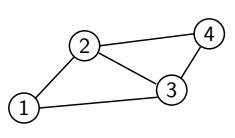
\includegraphics[scale=0.4]{grafo1_pequeno}

\end{figure}

\end{columns}

\vspace{.3cm}

Para o grafo da figura, assumindo $w_{ij} \in \{0, 1\}$ e $w_{ii} = 0$\\
$$ W = \begin{bmatrix}
0 & 1 & 1 & 0 \\ 
1 & 0 & 1 & 1 \\ 
1 & 1 & 0 & 1 \\ 
0 & 1 & 1 & 0
\end{bmatrix} \text{e }D = 
\begin{bmatrix}
2 & 0 & 0 & 0 \\ 
0 & 3 & 0 & 0 \\ 
0 & 0 & 3 & 0 \\ 
0 & 0 & 0 & 2
\end{bmatrix}  $$

\end{frame}

\begin{frame}{Grafos de similaridades e dissimilaridades}

O peso $w_{ij}$ é utilizado para representar algum tipo de relação entre os vértices $v_i$ e $v_j$

\begin{itemize}

\vspace{0.5cm}

\item Grafos de similaridade

\begin{itemize}

\item $w_{ij}$ representa a similaridade entre os dois vértices

\end{itemize}
\vspace{0.5cm}
\item Grafos de dissimilaridades (ou grafos de distância)

\begin{itemize}

\item $w_{ij}$ representa a dissimilaridade (ou distância) entre os dois vértices

\end{itemize}
\end{itemize}

\vspace{0.5cm}

Os dois modelos que iremos ver utilizam desses dois conceitos para agrupar pontos no espaço

\end{frame}

\begin{frame}{Construção de um grafo de similaridades a partir de pontos no $\R^p$}


Método da $\epsilon$-vizinhança

\begin{itemize}

\item Todos os pares de pontos no conjunto de dados cujas distâncias sejam menores que $\epsilon$ são conectados

\end{itemize}

Método dos $k$-vizinhos mais próximos

\begin{itemize}

\item Cada ponto no conjunto de dados é conectado aos seus $k$ vizinhos mais próximos

\end{itemize}

Método da função de similaridade

\begin{itemize}

\item Todos os pontos são conectados entre si, mas as similaridades entre cada par de pontos $w_{ij}$ é obtida segundo uma função \textit{Kernel} de similaridade $s: \R^p \times \R^p \rightarrow [0,1] $

\begin{itemize}
\item Exemplo: $ s(x_i, x_j) = exp(-\parallel x_i - x_j\parallel^2/(2\sigma^2))$
\end{itemize}

\end{itemize}


\end{frame}


\begin{frame}{Método da $\epsilon$-vizinhança - \textit{Iris}}

\vspace{0.3cm}

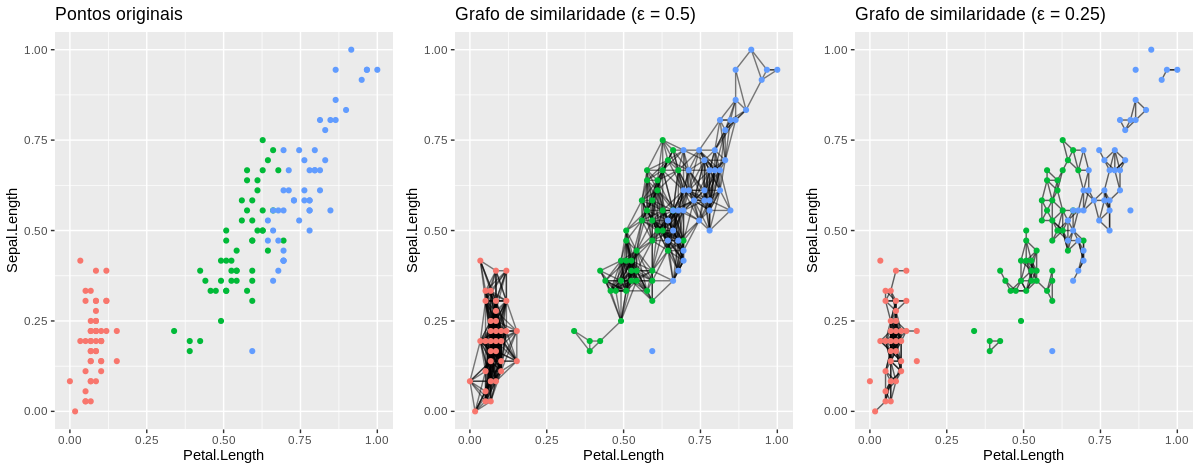
\includegraphics[scale=0.37]{epsilon_similarity}

\end{frame}

\begin{frame}{Laplaciano de um grafo}

O Laplaciano de um grafo ($L$) é uma matriz definida em termos de $W$ e $D$ que carrega propriedades importantes sobre o grafo. 

\vspace{0.3cm}

As definições de Laplacianos mais utilizadas são:

\begin{itemize}
\item Não normalizado: $L = D - W$
\vspace{0.3cm}
\item Normalizado: $L_{n} = D^{-1/2}LD^{-1/2}$
\vspace{0.3cm}
\item \textit{Random-walk}: $L_{rw} = I - D^{-1}W = I - P$

\begin{itemize}
\item Nesta definição, assume-se que $w_{ii} = 1$, para $i = 1, ..., n$ 
\vspace{0.4cm}
\item A matriz $P = D^{-1}W$ pode ser vista como a matriz de transição de um passeio aleatório no grafo $G$, onde $p_{ij} = \frac{w_{ij}}{d_i}$ 

\end{itemize}

\end{itemize}

\end{frame}

\begin{frame}{Propriedades principais do Laplaciano $L_{rw}$}

\begin{itemize}
\item $L_{rw}$ é simétrica e semi positiva definida

\vspace{.1cm}

\item O número de autovalores iguais a zero de $L_{rw}$ é igual ao número de conjuntos de vertices disjuntos não conexos.

\begin{figure}
\hspace*{2.3cm}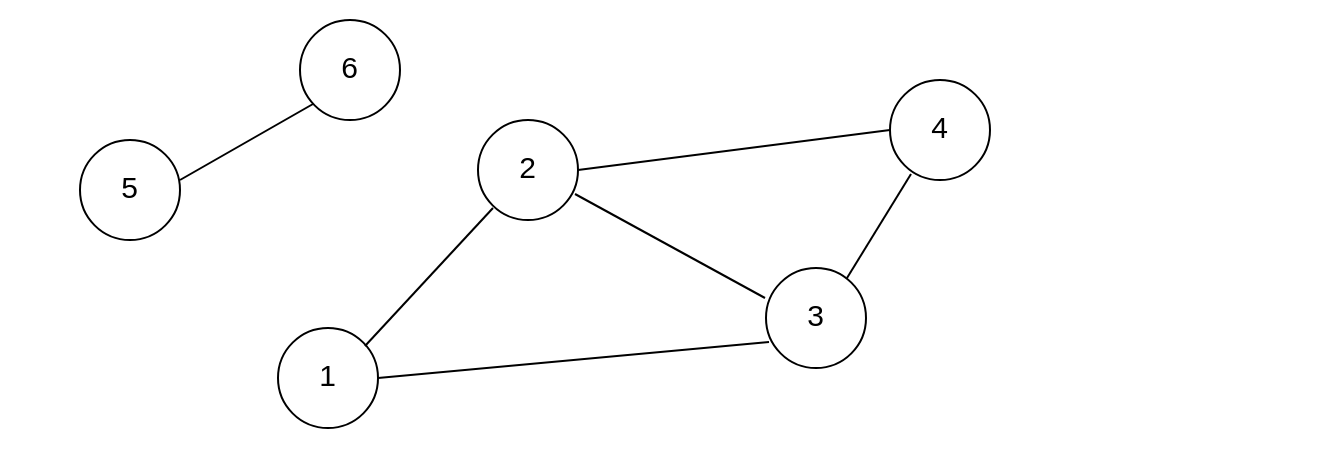
\includegraphics[scale=0.15]{grafo2_pequeno}
\caption{$\lambda_1 = \lambda_2 = 0$}
\end{figure}

\item  Se $u$ é um autovetor da matriz de transição $P$ do passeio aleatório $\Leftrightarrow$ $u$ é autovetor de $L_{rw}$

\begin{itemize}
\item Isso nos permite interpretar os autovetores de $L_{rw}$ em termos de distribuições
\end{itemize}

\end{itemize}


\end{frame}

\begin{frame}{Problema de agrupamento em termos de um passeio aleatório no grafo para}

Sejam $A_1, ..., A_k \subset V$ conjuntos disjuntos de vértices do grafo G. 

\vspace{0.3cm}

Definimos distribuição $\pi^{A}$ como 

$$\pi^{A}_i = \begin{cases} 1/|A|, & \text{se } i \in A \\ 0, & \text{caso contrário}\end{cases}$$

\vspace{0.5cm}

Procuramos $\pi^A$ que minimize a probabilidade do passeio aleatório sair ou entrar no conjunto $A$ , $C_A = P(A|A^C) + P(A^C|A)$

\vspace{0.5cm}

Pode ser provado que os k-primeiros autovetores de $L_{rw}$ são uma solução aproximada para o problema, relaxando-se algumas suposições sobre $\pi^A$

\end{frame}

\begin{frame}{Algoritmo de agrupamento espectral}

\begin{block}{Algoritmo de agrupamento espectral para pontos no $\R^p$}
\begin{enumerate}
\item Criar um grafo de similaridades entre os pontos do conjunto de dados 

\begin{itemize}
\item Usando o métodos da $\epsilon$-vizinhança, por exemplo
\end{itemize}

\vspace{0.5cm}
\item Calcular o Laplaciano $L_{rw} = I - D^{-1}W = I - P$

\vspace{0.5cm}

\item Extrair os $k$-primeiros autovetores de $L_{rw}$, excluindo-se o primeiro autovetor

\vspace{0.5cm}

\item Aplicar o método das K-médias na matriz de dados dos $k$-autovetores extraidos

\end{enumerate}
\end{block}

\end{frame}

\begin{frame}{Exemplos}
\begin{enumerate}

\item Do conjunto de dados de 373 pontos no $\R^2$, utilizando o método da $\epsilon$-vizinhança, obtemos um grafo de similaridades

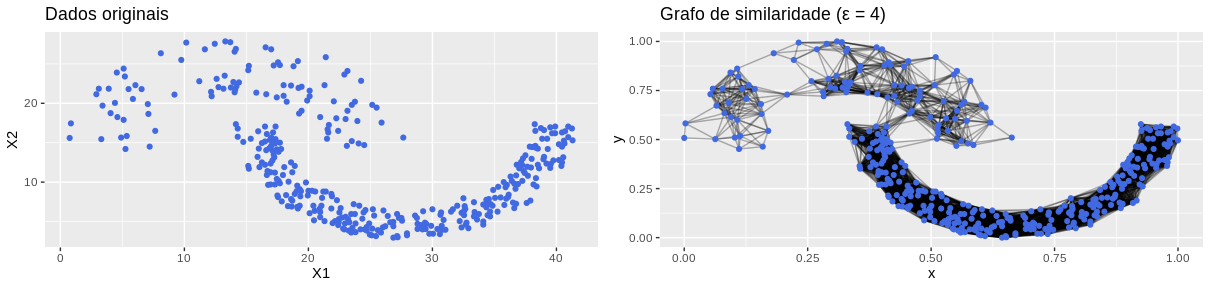
\includegraphics[scale=0.34]{horse}

\item Obtemos os 2 primeiros autovetores de $L_{rw}$. Após descartar o primeiro autovetor, ficamos com o segundo autovetor

\end{enumerate}

\end{frame}

\begin{frame}
\begin{enumerate}
\setcounter{enumi}{2}

\item Aplicamos o método das $K$-médias (com $K$ = 2) nos valores do segundo autovetor

\vspace{1cm}

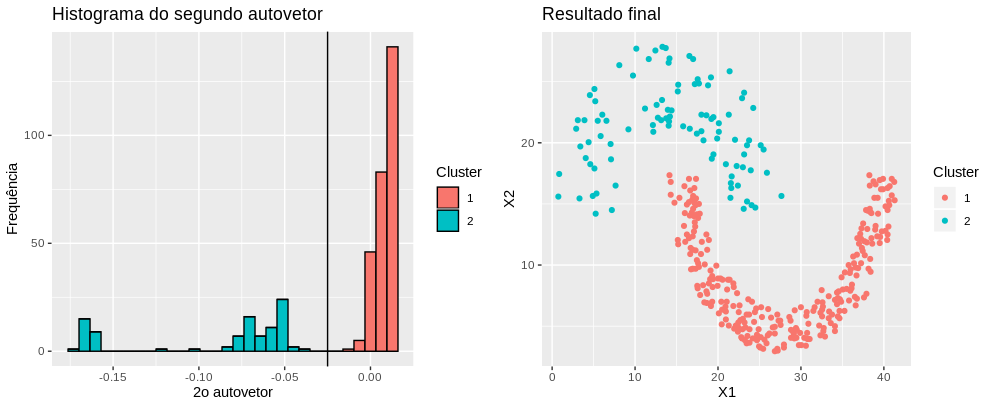
\includegraphics[scale=0.4]{final}

\end{enumerate}
\end{frame}

\begin{frame}{ISOMAP}

\begin{itemize}

\item Alguns métodos alternativos exploram o conceito de grafos de dissimilaridade (distâncias)

\vspace{1cm}

\item O algoritmo ISOMAP, assim como o modelo de agrupamento espectral, cria um grafo a partir de pontos espalhados no $R^p$ (usando algum dos três métodos que vimos acima). 

\item A diferença é que os pesos das arestas $w_{ij}$ são definidos como a distância euclidiana entre os dois pontos $x_i$, $x_j$. Isto é,

$$w_{ij} = \parallel x_i - x_j\parallel^2$$

\end{itemize}

\vspace{.5cm}

\end{frame}

\begin{frame}{Distância geodésica em um grafo}

\begin{block}{Caminho possíveis entre dois vértices}
Seja $C_{ij}$ o conjunto de caminhos possíveis no grafo partindo-se do vértice $v_i$ ao vértice $v_j$.
\end{block}

\vspace{0.5cm}

A distância geodésica entre dois vértices $v_i$ e $v_j$ é definida como a distância percorrida do menor caminho possível unindo $v_i$ e $v_j$, isto é

\begin{columns}

\column{0.6\textwidth}

$ d(i, j) = min_{ K \in C_{ij} } \left (\sum_{(k_1 - k_2) \in K} w_{k_1k_2} \right )$

\column{0.3\textwidth}

\vspace{0.5cm}

\begin{figure}
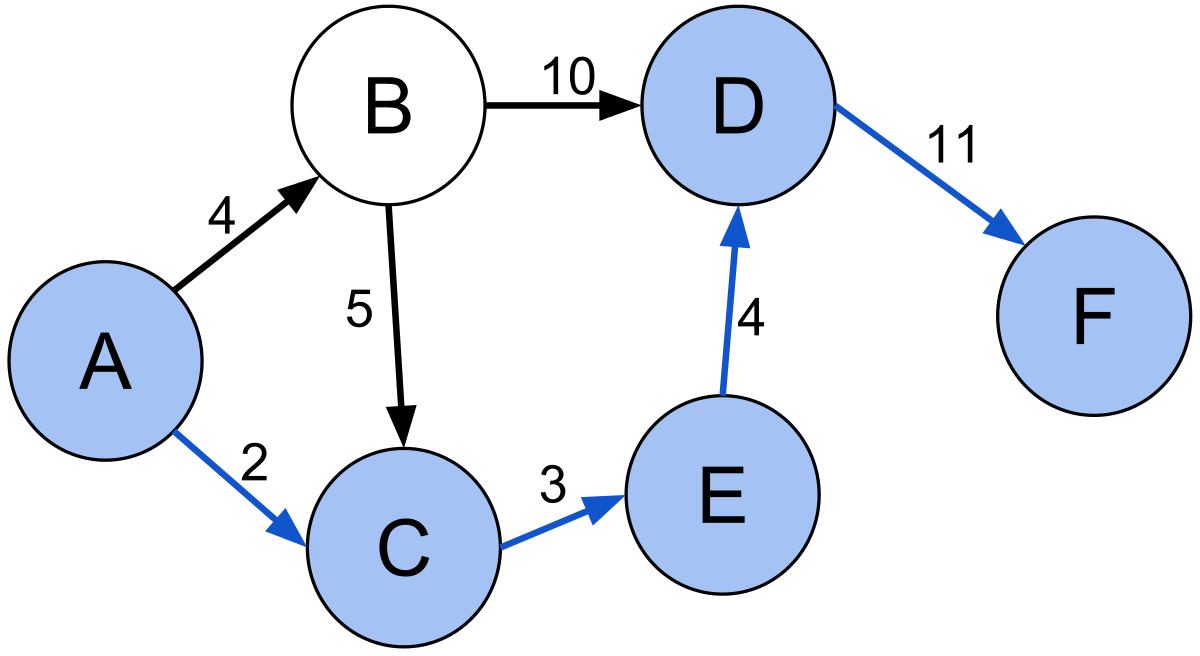
\includegraphics[scale=0.07]{geodesic}
\end{figure}


\vspace{.5cm}
\end{columns}


\end{frame}

\begin{frame}{ISOMAP}

\begin{block}{Algoritmo}
\begin{enumerate}
\item Criar um grafo de distâncias entre os pontos do conjunto de dados 

\begin{itemize}
\item Usando o métodos da $\epsilon$-vizinhança, por exemplo
\item Os pesos $w_{ij}$ dos vértices que foram conectados assumem o valor da distância euclidiana entre estes dois pontos, $d(x_i, x_j)$
\end{itemize}

\vspace{0.2cm}
\item Obter a matriz de distâncias geodésicas $D_{nxn}$

\vspace{0.5cm}

\item Extrair coordenadas principais de $D_{nxn}$ usando Escalonamento Multidimensional

\vspace{0.5cm}

\item Aplicar o método das K-médias nos pontos projetados nas coordenadas principais

\end{enumerate}
\end{block}

\end{frame}

\begin{frame}{Exemplo}

\hspace*{1.5cm}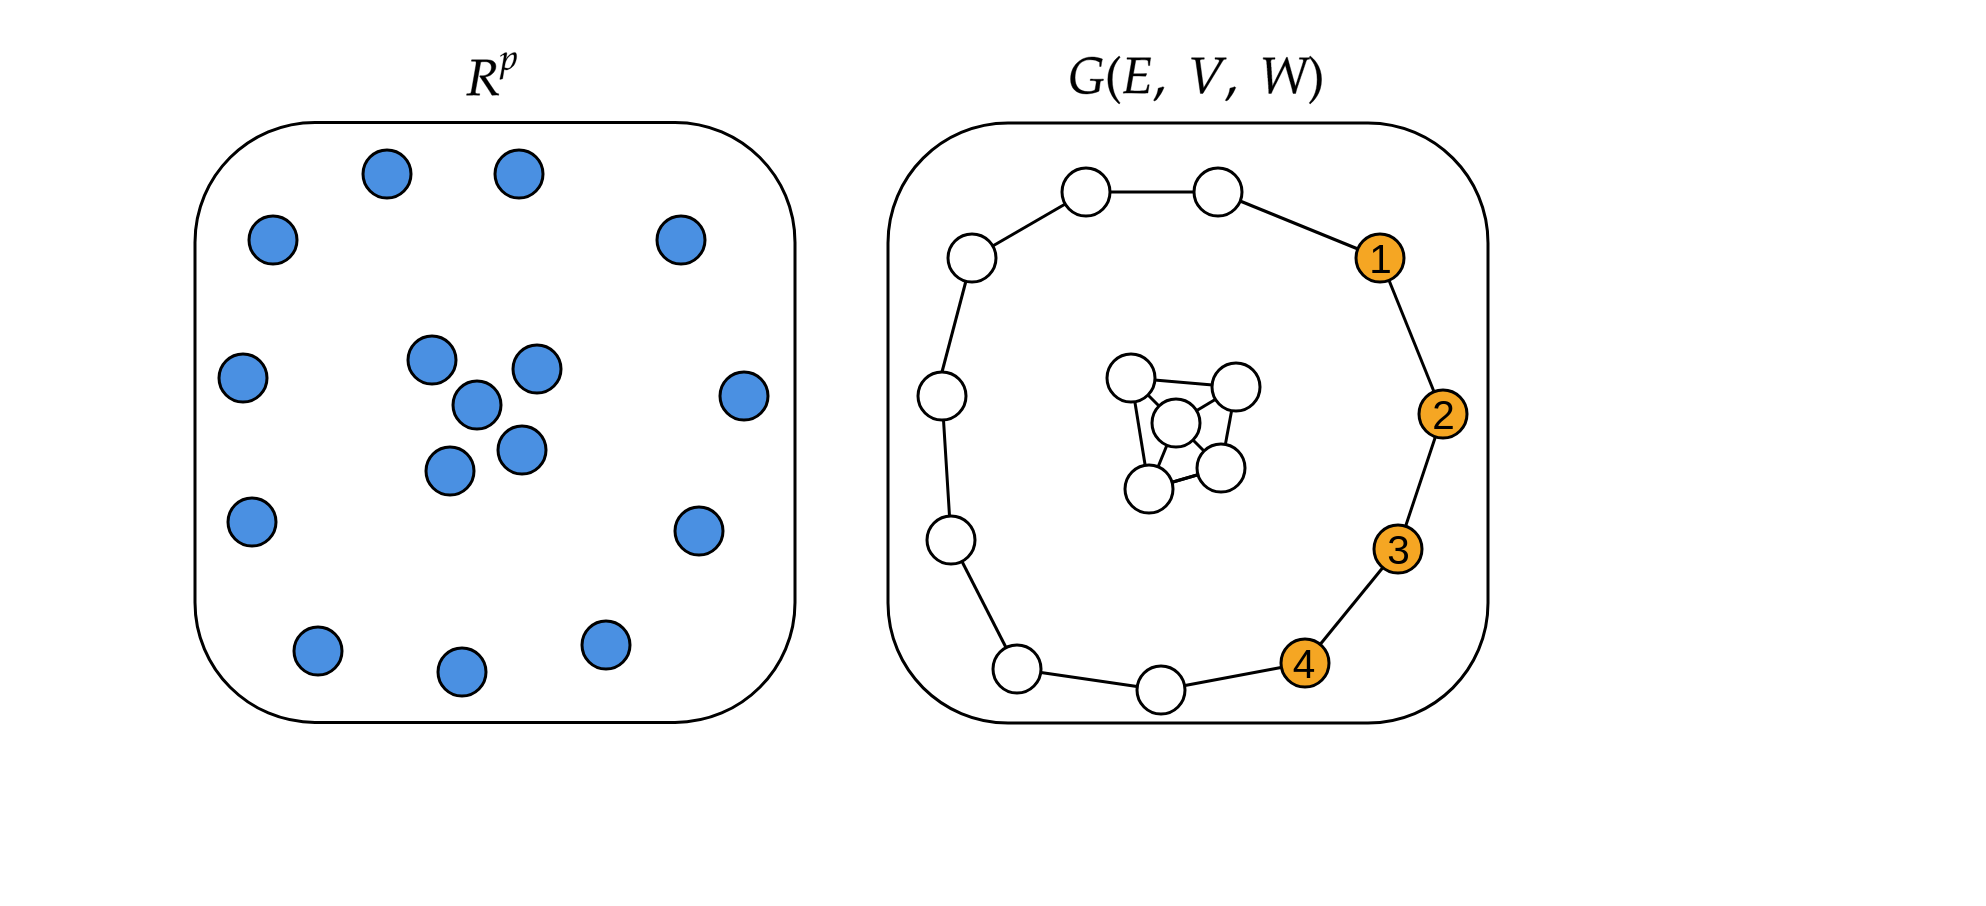
\includegraphics[scale=0.15]{iso3}

A distância geodésica entre os vértices 1 e 4 é 
$$w_{12} + w_{23} + w_{34} = d(x_1, x_2) + d(x_2, x_3) + d(x_3, x_4)$$

\end{frame}

\begin{frame}{Exemplo}

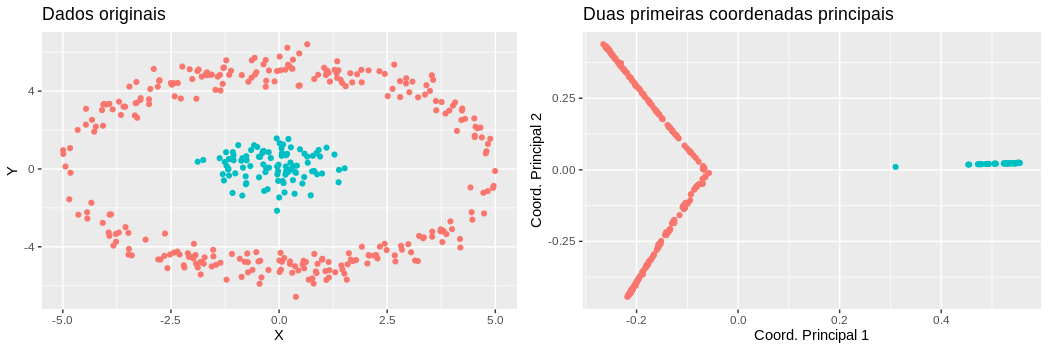
\includegraphics[scale=0.42]{isomap_result}

\end{frame}

\begin{frame}{Referências}

\begin{enumerate}
\item Luxburg, U. (2007), \textit{A Tutorial on Spectral Clustering}

\vspace{1cm}

\item Lovàsz, L. (1993). \textit{Random walks on graphs: A Survey}

\vspace{1cm}

\item Tenenbaum, J. (2000). \textit{A Global Geometric Framework for Nonlinear Dimensionality Reduction}
\end{enumerate}

\end{frame}

\end{document}